\documentclass{article}
\usepackage{listings}
\usepackage{geometry}
\usepackage{amsmath,amsthm,amssymb}
\usepackage{hyperref}
\usepackage{color}
\usepackage{mathtools}
\usepackage{tikz-cd}

% mathbb shortcuts
\newcommand{\Z}{\mathbb{Z}}
\newcommand{\N}{\mathbb{N}}
\newcommand{\Q}{\mathbb{Q}}
\newcommand{\R}{\mathbb{R}}
\newcommand{\C}{\mathbb{C}}
\newcommand{\F}{\mathbb{F}}
\newcommand{\T}{\mathbb{T}}
\newcommand{\HH}{\mathbb{H}}
\newcommand{\RP}{\mathbb{RP}}
\newcommand{\PP}{\mathbb{P}}
\newcommand{\A}{\mathbb{A}}
\newcommand{\E}{\mathbb{E}}

% mathfrak shortcuts
\newcommand{\fI}{\mathfrak{I}}
\newcommand{\fA}{\mathfrak{A}}
\newcommand{\fG}{\mathfrak{G}}

% mathcal shortcuts
\newcommand{\cA}{\mathcal{A}}
\newcommand{\cU}{\mathcal{U}}
\newcommand{\cR}{\mathcal{R}}
\newcommand{\cP}{\mathcal{P}}
\newcommand{\cB}{\mathcal{B}}
\newcommand{\cC}{\mathcal{C}}
\newcommand{\cF}{\mathcal{F}}

\newcommand{\Aut}{\textrm{Aut}}
\newcommand{\degg}{\textrm{deg}}
\newcommand{\Hom}{\textrm{Hom}}
\newcommand{\conj}{\textrm{conj}}
\newcommand{\Gal}{\textrm{Gal}}
\newcommand{\disc}{\textrm{disc}}
\newcommand{\supp}{\textrm{supp}}
\newcommand{\Jac}{\textrm{Jac}}
\newcommand{\Der}{\textrm{Der}}
\newcommand{\Spec}{\textsf{Spec}\,}
\newcommand{\im}{\textrm{im}\,}

% mathsf shortcuts
\newcommand{\Cell}{\textsf{Cell}}

\newcommand{\clr}{\color{red}}


\begin{document}

\begin{center}
	\large \textbf{GRST Notes: Examples of Sheaf Cohomology (November 2, 2016)} \\
\end{center}


We move on to a discussion of some simple examples of sheaf cohomology. The goal here will be to first compute the cohomology groups explicitly, and then try and figure out a more intuitive idea of what is going on behind each cohomology group. We’ll start with the triangle cell complex, denoted $X$, that we considered in the last post.

\begin{figure}[!htbp]
\centering
	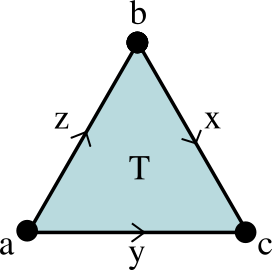
\includegraphics[width=0.15\textwidth]{triangle_dir.png}
\end{figure}

We will consider the constant sheaf $F_0$ over the triangle, where we assign a 1-dimensional vector space $k$ over each cell, and every map is an identity map. To be explicit, the diagram of the sheaf will look like the following

\[
\begin{tikzcd}
	& k & \\
	k \arrow{ur} & k \arrow{u} & k \arrow{ul} \\
	k \arrow{ur} \arrow{urr} & k \arrow{ur} \arrow{ul} & k \arrow{ul} \arrow{ull}
\end{tikzcd}
\]

where each arrow represents the identity map. The bottom row represents the vertices, the middle row represents the edges, and the top row represents the face. Thus, the co-chain complex for this sheaf would be

\begin{equation}
	0 \xrightarrow{} k^3 \xrightarrow{\delta^0} k^3 \xrightarrow{\delta^1} k \xrightarrow{\delta^2}  \ldots
\end{equation}

Note that the boundary maps are maps between vector spaces, we can write out each boundary map as a matrix. We will label the basis vectors of each vector space by the corresponding cell with a hat. For example, the set of ordered basis vectors is $\{\hat{a},\hat{b},\hat{c}\}$ for $C^0(X;F_0) = k^3$, $\{\hat{x},\hat{y},\hat{z}\}$ for $C^1(X;F_0) = k^3$ and $\{\hat{T}\}$ for $C^2(X;F_0)$. Recall from the previous post that the differential is defined by

\begin{equation}
	\delta^k = \sum_{\sigma \leq_1 \tau} [\sigma^k : \tau^{k+1}] \rho_{\tau, \sigma}.
\end{equation}

We can think of the formula in the summand as the $\hat{\sigma}, \hat{\tau}$ element of the matrix representation of $\delta_k$. Then, the $\delta_0$ and $\delta_1$ maps for this example have the following matrix representations.
\begin{equation}
	\delta^0(X;F_0) = \begin{pmatrix} 0 & 1 & -1 \\ 1 & 0 & -1 \\ 1 & -1 & 0 \end{pmatrix}
\end{equation}
\begin{equation}
	\delta^1(X;F_0) = \begin{pmatrix} 1 & -1 & 1 \end{pmatrix}
\end{equation}

From these matrix equations, it is simple to compute the kernel and image of the differential maps to get the following:
\begin{equation}
	\ker \delta^0 = \langle \hat{a} + \hat{b} + \hat{c} \rangle \hspace{20pt} \im \delta^0 = \langle \hat{y} + \hat{z}, \hat{x} - \hat{z} \rangle
\end{equation}
\begin{equation}
\ker \delta^1 = \langle \hat{y} + \hat{z}, \hat{x} - \hat{z} \rangle \hspace{20pt} \im \delta^1 = \langle \hat{T} \rangle
\end{equation}

Finally, the cohomology groups are computed as the following.
\begin{equation}
H^0 (X; F_0) = \ker \delta^0 = k
\end{equation}
\begin{equation}
H^1 (X; F_0) = \frac{\ker \delta^1}{\im \delta^0} = 0
\end{equation}
Note that in this example, the intermediate steps of calculating the sheaf cohomology groups coincide with those of calculating the singular cohomology groups of the triangle.\\

However, sheaf cohomology doesn't just depend on the underlying cell complex; it also depends on the choice of sheaf. Here we will consider the same triangle cell complex X but define the sheaf differently.

\begin{figure}[!htbp]
\centering
	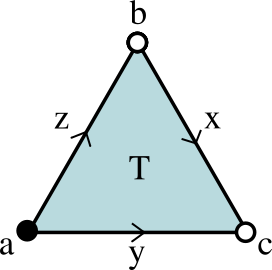
\includegraphics[width=0.15\textwidth]{triangle_dir_bc.png}
\end{figure}

Similar to the previous example, we assign each cell a 1-dimensional vector space $k$ and assign each map to be the constant map except those from cell $b$ or $c$ (the hollowed out vertices in the figure). The maps from these cells will be the zero map. We denote this sheaf to be $F_1$, and the diagram can be seen in the next figure, where the balck arrows represent identity maps and the red arrows represent zero maps.

\[
\begin{tikzcd}
	& k & \\
	k \arrow{ur} & k \arrow{u} & k \arrow{ul} \\
	k \arrow{ur} \arrow{urr} & k \arrow[red]{ur} \arrow[red]{ul} & k \arrow[red]{ul} \arrow[red]{ull}
\end{tikzcd}
\]

Following the same procedure as the first example, we can calculate the matrices representing the boundary maps for this cellular sheaf.
\begin{equation}
	\delta^0(X;F_1) = \begin{pmatrix} 0 & 0 & 0 \\ 1 & 0 & 0 \\ 1 & 0 & 0 \end{pmatrix}
\end{equation}
\begin{equation}
	\delta^1(X;F_1) = \begin{pmatrix} 1 & -1 & 1 \end{pmatrix}
\end{equation}

Continuing the procedure, we calculate the images and kernels.

\begin{equation}
	\ker \delta^0 = \langle \hat{a}, \hat{b} - \hat{c} \rangle \hspace{20pt} \im \delta^0 = \langle \hat{y} + \hat{z} \rangle
\end{equation}
\begin{equation}
\ker \delta^1 = \langle \hat{y} + \hat{z}, \hat{x} - \hat{z} \rangle \hspace{20pt} \im \delta^1 = \langle \hat{T} \rangle
\end{equation}

Finally, we can use this to compute the cohomology groups.
\begin{equation}
H^0 (X; F_0) = k^2, \hspace{20pt} H^1(X; F_1) = k
\end{equation}

Here we can see that even though the cell complex underlying both examples was the same, the resulting cohomology groups is dependent on the choice of sheaf. This shows that we can’t just use our intuition from simplicial or singular cohomology when dealing with sheaf cohomology. The goal is to come up with some intuition for what the cohomology groups should be given some pictorial representation of the sheaf (such as the images of the triangles above).\\

We can think of the zeroth cohomology group as representing the global sections of the sheaf. A global section is a choice of an element from each object in the sheaf such that it is consistent with all of the maps. For example, consider the diagram of the constant sheaf, and suppose our vector space is simply $k = \R$. Then, choosing a number $r \in \R$ for any of the vector spaces would uniquely determine the choices for all other vector spaces due to the required consistency with the identity mapping. Hence, the cohomology group of $H_0(X;F_0) = k$ is consistent with the number of global sections for the constant sheaf.\\

Next we consider the sheaf $F_1$, where the maps out of b and c are the zero maps. In the following diagram, the objects represent a choice of element in each vector space. Note that these zero maps, along with the fact that all other maps are the identity, will force all vector spaces other than those associated with $b$ and $c$ to have the element 0.

\[
\begin{tikzcd}
	& 0 & \\
	0 \arrow{ur} & 0 \arrow{u} & 0 \arrow{ul} \\
	0 \arrow{ur} \arrow{urr} & b \arrow[red]{ur} \arrow[red]{ul} & c \arrow[red]{ul} \arrow[red]{ull}
\end{tikzcd}
\]

Here, the red arrows (the zero maps) force the vector spaces in the middle row to have the element 0, and all vector spaces connected to the middle row by black arrows (the identity map) must also take the element 0. Thus, we are left with independent choices for b and c. Again, the cohomology group of $H_0(X; F_1) = k^2$ is consistent with the number of global sections for this sheaf.

\end{document}